\documentclass[letterpaper]{article}
% DO NOT CHANGE THIS
\usepackage{aaai24} % DO NOT CHANGE THIS
\usepackage{times} % DO NOT CHANGE THIS
\usepackage{helvet} % DO NOT CHANGE THIS
\usepackage{courier} % DO NOT CHANGE THIS
\usepackage[hyphens]{url} % DO NOT CHANGE THIS
\usepackage{graphicx} % DO NOT CHANGE THIS
\urlstyle{rm} % DO NOT CHANGE THIS
\def\UrlFont{\rm} % DO NOT CHANGE THIS
\usepackage{graphicx}  % DO NOT CHANGE THIS
\usepackage{natbib}  % DO NOT CHANGE THIS
\usepackage{caption}  % DO NOT CHANGE THIS
\frenchspacing % DO NOT CHANGE THIS
\setlength{\pdfpagewidth}{8.5in} % DO NOT CHANGE THIS
\setlength{\pdfpageheight}{11in} % DO NOT CHANGE THIS
%
% Keep the \pdfinfo as shown here. There's no need
% for you to add the /Title and /Author tags.
\pdfinfo{
/TemplateVersion (2024.1)
}

\setcounter{secnumdepth}{0} %May be changed to 1 or 2 if section numbers are desired.

\usepackage{cleveref} % custom addition for easy figure references

\title{Shepherd: An Incremental Story Sifting-Based Drama Manager}
\author {
    Sage Deo,
    Jonathan Chung,
    Joshua McCoy
}
\affiliations {
    University of California, Davis \\
    \{rsdeo, jonchung, jamccoy\}@ucdavis.edu
}

\begin{document}
\maketitle

\begin{abstract}
    Incremental story sifters analyze an in-progress simulation to extract interesting
    narrative content or find a set of events that have the \textit{potential} to become
    more narratively interesting if followed up in a certain way. There has been some
    investigation on the potential for an incremental story sifter to suggest future
    narrative events to human authors, but the technique of guiding a simulation using
    story sifting, without any human interference, remains completely unexplored. Thus, we
    present Shepherd, a drama manager powered by incremental story sifting, which guides
    otherwise completely autonomous characters toward making narratively interesting
    choices. 
\end{abstract}

\section{Introduction}
In the field of interactive emergent narrative, there is a distinction made between a
chronicle of simulated events and a narrative. The key element that transforms a chronicle
into a narrative is curation, the process of cutting out narratively irrelevant content
from a chronicle to create a narrative. However, this raises an important question: how do
we decide which parts of a chronicle constitute a narrative?

Oftentimes, as in the case of \textit{Bad News} \cite{samuel:badnews}, humans are able to
intuitively find small sequences of narratively interesting content, and then assemble
those sequences into a larger narrative. This process has been termed “story sifting.” To
aid in automatic narrative curation, automatic story sifters such as Felt
\cite{kreminski:felt} and Sheldon \cite{ryan:curating} were created. These automatic story
sifters accept human-authored “story templates,” which are high-level descriptions of
small sequences of narratively interesting material. Given a chronicle of simulated events
and a set of story templates, automatic story sifters can identify themes such as
“violation of hospitality” or “repeated betrayals,” which can later be assembled into a
narrative. 

Later, the notion of “incremental story sifting” was implemented in Winnow
\cite{kreminski:winnow}, the successor
language to Felt. Winnow is capable of identifying partially-fulfilled story templates in
a simulation currently in progress, which the authors note could potentially be used for
foreshadowing future plot developments, i.e. the completion of the partially-filled
template in question. However, this also opens up the possibility of using Winnow, or any
other incremental story sifter, as a sort of drama manager to guide a simulation in
progress towards making choices that progress any partially-filled story templates it
detects. This was explored to some degree by \textit{Loose Ends} \cite{kreminski:loose}, a mixed-initiative authoring
system which uses Winnow to suggest plot developments for a human to choose between.
However, this technique has not yet been explored as part of a fully autonomous
simulation, without any human guidance. 

In this work, we contribute the Shepherd system, the first (to our knowledge) instance of
a story sifter being leveraged for drama management in a simulation with no human input.
Shepherd differs from other story sifters due to the fact that it sifts alongside the
generator, allowing our system to have focused, curated narratives alongside the variance
of a chaotic generator. It nudges the course of the narrative rather than outright
demanding that certain events take place, allowing our system to follow story structures
in interesting ways while still retaining a degree of control and coherence. The
creativity and cohesion of the stories our system will generate will be proof that this
method of incremental story sifting alongside generation is a viable and ripe path to
pursue.

\section{Related Work}
This work is very informed by \textit{Curating Simulated Storyworlds} \cite{ryan:curating} and its
philosophy on story sifting and emergent narrative, especially as that philosophy is
instantiated in the theatrical performance piece \textit{Bad News}. We also directly use the Winnow
incremental story sifter in our implementation of this system. Our
use of story sifting as a drama manager, to guide a simulation in progress, is a
simulationist extension of its use in the \textit{Loose Ends} system. 
% TODO: a versu citation should go here
Where
\textit{Loose Ends} is a “strong story” system, in which a story sifter acts to guide a human
author with ultimate control over the plot, our proposed system takes a “strong autonomy”
approach, where the story sifter guides the characters, who otherwise make their own
decisions. 

Guided by the work of Max Kreminski, Noah Wardrip-Fruin, and Michael Mateas in
\textit{Authoring For Story Sifters} \cite{kreminski:authoring}, we intend to address the
most glaring issue with interactive emergent narrative: “the dissolution of the
player-perceived story into a structureless mess”. While Shepherd characters make their
own decisions, they are guided by the drama manager to advance and complete story arcs. By
sifting simultaneously with generation, Shepherd provides structure to the story itself
rather than looking for narratives post-generation as the wizard of \textit{Bad News} does.
Although this sacrifices some randomness and chaos during the generation phase, the
corresponding reward of coherence is far more impactful. In addition, because Shepherd
remains a “strong autonomy” system, the characters continue to make decisions and create
stories that surprise. As a result, Shepherd will generate stories that deviate from the
established story templates which players will narrativize themselves as they do in
\textit{Dwarf Fortress} or \textit{The Sims}.
% TODO: cite DF/Sims?

\section{Technical Description}
The basic building blocks of a Shepherd world are time, characters, actions, traits, and
templates. The interactions between all of these pieces, as well as the drama manager,
form the basis for rich emergent stories.

\subsection{Time}
In Shepherd, time is divided into a series of discrete time steps. For each time step,
each character in the simulation may perform one action. For ease of computation, all
actions are internally represented as taking place in sequence. However, readers may
construct narratives in which actions within the same time step happen in parallel. This
openness to interpretation helps facilitate narrativization.

\subsection{Characters}
Characters in Shepherd are mostly-autonomous agents. Every time step, each character
generates a utility score for each possible action they can take, based on that
character's traits. The utility score is combined with the drama manager's score for that
action to produce an overall score. Then, the character makes a weighted random choice
between all possible actions, with each action's overall score used as its weight.

This method of modeling character decisions allows for character choices to follow
consistent trends, which is good for allowing the audience to understand each character.
However, it also allows characters to infrequently surprise the audience, creating
narrative intrigue.

\subsection{Actions}
An action is an event in the story world that can be triggered by some character (the
actor). Some actions are monadic, and have only an actor; however, other actions are
dyadic, and involve a separate character who is not the actor (the target). Each character
may only serve as the actor for one action per time step, but each character can serve as
the target for arbitrarily many actions per time step.

Each action also has a set of tags that provide higher-level information about each event:
some examples of tags are ``friendly,'' ``food,'' and ``violent.'' Tags mainly interact
with the rest of the system in two ways. First, when evaluating an action (via their
traits), characters consider that action's tags when determining its utility score.
Second, human-authored story templates can match actions based on tags. This allows a
single line in a pattern to represent a wide variety of actions which are all narratively
equivalent in the context of that pattern.

\subsection{Traits}
Traits are the main agents of character personality modeling, and provide the basis for
utility-based character decision-making. Each character is assigned a consistent number of
(currently, two) traits at character generation, and each trait has its own utility
function. A character's utility score for a given action is the sum of the utility scores
for each of the character's traits evaluated on that action. At a high level, this means
that each character is likely to act in ways that are consistent with each of their
traits: for example, a character who is friendly (high utility for actions tagged
``friendly'') and a gourmet (high utility for actions tagged ``food'') is very likely to want to
share a meal with some other character, because sharing a meal is tagged as both
``friendly'' and as ``food.'' 

\begin{figure}[h]
    \centering
    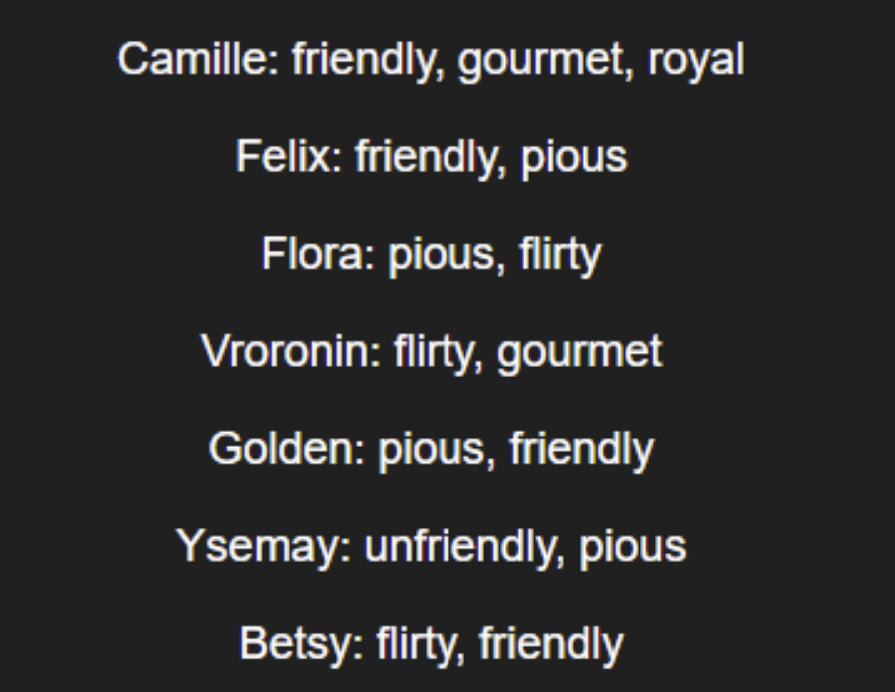
\includegraphics[width=\columnwidth]{figure-traits}
    \caption{A screenshot from the Shepherd UI, showing each character's name and traits.}
    \label{fig:traits}
\end{figure}


Like tags, traits can also be used as conditions when writing templates. Thus, one
character's traits may influence other characters' behavior via the drama manager.

\subsection{Templates and the Drama Manager}
Each template represents a sequence of narratively interesting events, such as a ``drunken
brawl'' or ``failed flirtation.'' Templates are expressed as patterns in the Winnow
language. Shepherd maintains a list of possible, partially filled, and complete templates;
this list is updated each time an action is taken. Furthermore, when the drama manager
evaluates an action, it checks to see if that action would advance any of its tracked
story templates. Actions that advance many story templates are valued more highly by the
drama manager, as are actions that advance story templates which are close to completion.
This makes it more likely that characters take actions that are narratively interesting
and which work towards resolving open plot threads.

% TODO: add more?

\section{Analysis}
Shepherd successfully straddles the line between structure and chaos in its generation.
The following example of one of Shepherd’s outputs demonstrates its ability to produce
comparable amounts of variability to other interactive emergent narrative systems while
simultaneously providing recognizable structures and coherence. \Cref{fig:traits} shows the
traits of the characters in this specific simulation. Just as in Bad News, refreshing or
closing this tab destroys this particular simulation, granting it a certain ethereality;
although, of course this simulation will enjoy greater longevity due to its presence in
this paper.

Because the only way for the player to understand and get a sense for the personality of a
character is through their actions and the traits, it becomes imperative that the
characters act according to their traits. Shepherd succeeds here as the actions of the
characters do line up with the traits that they are assigned. \Cref{fig:eat} is the
very first line of this simulation which shows Camille’s tendency to choose more actions
tagged “eat.”

\begin{figure}[h]
    \centering
    
\includegraphics[width=\columnwidth]{figure-cf_eat}
    \caption{An example of an action choice influenced by Camille's ``friendly'' and
    ``gourmet'' traits.}
    \label{fig:eat}
\end{figure}

But characters don’t necessarily have to follow their traits. They deviate frequently from
their traits, doing things randomly or to fulfill set story templates. However, the
display of the traits themselves may alter the perception of the player and how they may
narrativize events. For example, in \cref{fig:bite} Betsy randomly chooses the “violent”
and “unfriendly” action of biting Camille. This runs contradictory to the established
“friendly” trait for Betsy, but due in part to Camille’s reaction and to Betsy’s “flirty”
trait the event can be narrativized by players in its new context. Thus, the traits of
characters in Shepherd do a great deal to color the perceptions of their actions.

\begin{figure}[h]
    \centering
    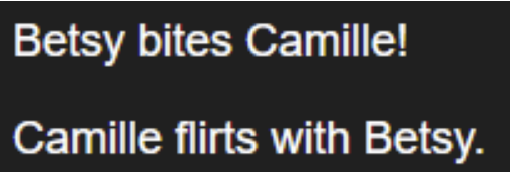
\includegraphics[width=\columnwidth]{figure-bc_bite_flirt}
    \caption{An example of a surprising choice arising from Shepherd's algorithm for
    character decision-making, which players can narrativize in interesting ways.}
    \label{fig:bite}
\end{figure}

\Cref{fig:pray} demonstrates the power of incremental story sifting
alongside generation. Shepherd successfully nudges characters to pick actions that advance
or complete story arcs, which allows for more satisfying consequences and results for
actions and alleviates the “structureless mess.” Shepherd can handle and track any number
of story templates which allows for the tracking and conclusion of multiple arcs at a
time. The successful completion of story arcs with clear beginning, middle, and ends
provides catharsis and a sense of logical progression. 

\begin{figure}[h]
    \centering
    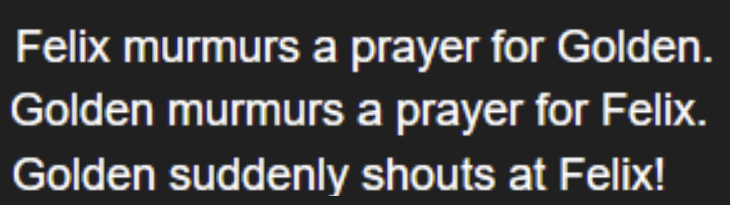
\includegraphics[width=\columnwidth]{figure-fg_pray_shout}
    \caption{An example of how Shepherd's story templates result in more structured story
    arcs. This series of actions took place over multiple time steps.}
    \label{fig:pray}
\end{figure}

\section{Conclusion}
We have introduced Shepherd, an incremental story sifting-based drama manager that guides
simulations towards producing interesting narratives. Shepherd represents a completely new
application of story sifting which is ripe for further exploration and evaluation. The
system is very easy to author for, is extremely scalable and extensible, and results in
the emergence of surprising and interesting character behavior from otherwise unstructured
simulation, while still leaving room for players to narrativize. We hope that, in the
future, this new paradigm can aid in the creation of interactive digital narratives that
offer the usual pleasures of emergent narrative while minimizing some of the associated
pains.

\subsection{Future Work}
There are many possible ways to expand on the work presented here. Shepherd itself can be
improved in many ways: we hope to expand the state-tracking capabilities of the system so
that, for example, character relationships can be better modeled and act as narrative
material. We also hope to create authoring tools to make writing for Shepherd easier,
especially for authors who may not be well-versed in programming. 

There is also work to be done to properly evaluate Shepherd, both from the perspective of
authors writing for Shepherd and players experiencing the resulting narratives. From the
author perspective, it may be wise to conduct a user study, especially once the
aforementioned authoring tools have been implemented. From the player perspective, another
user study might help evaluate the interestingness of simulations guided by Shepherd. To
fully evaluate Shepherd in production, we also hope to mount it in a fully realized
narrative game, with graphical output and increased player interactivity. 

Lastly, one shortcoming of Shepherd is that, though it generates character actions that
follow predetermined story templates, the arc of each story may be hard for players to
discern. This is true of most or all simulation-based systems, but Shepherd is unique in
that it constantly tracks the progress of each story arc; thus, it is uniquely positioned
to make this information more accessible to players. One potential way of doing so is
inspired by \textit{Loose Ends}: in that system, each action that progresses a story goal
is associated with some text that situates that action in the context of the story goal in
question. A similar approach could be integrated with Shepherd to contextualize each
action with respect to all story templates progressed by that action. User interface
changes may also help make story arcs more apparent by drawing a better continuity between
each character's actions, or even allowing players to see only the parts of the simulation
that pertain to a specific character.

\bibliography{refs}

\end{document}
